
\documentclass[twocolumn, amsmath]{revtex4}

\usepackage{graphicx}
%\graphicspath{ {tex_pics/} }


\begin{document}


\title{PHYS 605 Lab \#6} 

\author{Morgan A. Daly}
\author{Evin O'Shea}
\date{\today} 


\maketitle


\section{Introduction and Theory}
\subsection{Purpose}

The goal of part A of the lab was to investigate the internal resistance of the protoboard's AC voltage supply. This was a good practice in measuring the output voltage and output impedance of a circuit. 
Part A of the lab gave practice for part B of the lab which was to investigate the output impedance of an op amp circuit. In this case the circuit was an inverting amplifier with a gain of three. Along with output impedance, the limitations of possible loads and the affects of differentt resistor values in the op amp circuit.
Part C of the lab was to build a differen op amp circuit. The lab group chose to build a high pass filter and amplifier. This circuit's nature was investigated by measuring output voltage versus input frequency. The plot of this relationship will show the nature of the filter.

\subsection{Background / Theory}

Output impedance and voltage of a circuit is important to know. When a voltage is being supplied from an active circuit to a load, the output impedance can tell a lot about the limitations of the loads that can be used. If the outpuyt impedance fo a passive circuit is much higher than the impedance of the circuit load, then sag can occur. This will mean that the circuit will not work as desired. The magnitude of the output impedance of a circuit can be measured by measureing the ouput voltage of a circuit with no load, and then measuring the ouput voltage with a load. The output impedance in voltage can be described by the thevenin equivalent of the circuit. The thevenin voltage is measured when th output voltage is measured without the load. WHen the load is applied, knowing the load resisitance and the voltage across the load will give the nortan current. Together, the thevenin voltage and nortan current can give the output impedance
Op amps are acitve circuit elements that can be used in a multitude of ways. The most important property of an op amp is that the positive and negative terminals of the op amp will be equal. This means that since the positive terminal is grounded, the voltage of the positive and negative terminal will both be zero.
The invertive amplifier built for this lab is shown below:

this circuit blah blah (how it works)

For the third part of the lab, a high pass filter and amplifer was made with the op amp. This circuit is shown below. This circuit is a high pass filter because the capacitor only allows high freqency voltages to pass through. In a DC circuit, a capacitor will simply be charged and no current will flow after. In an AC cuircuit, changes in the voltage across the capacitor on one side will cause changes in voltage on the other side. This will allow the AC current to flow through the capacitor. Since the capacitor responds to changes in voltage, higher freqency voltages will pass through the circuit mor easily than low frequency voltages. This is the reason that a circuit in this situation will act as a high pass filter. In this circuit, since there is a negative feedback, the postivie and negative terminals of the op amp will have an equal voiltage. Again, since the positive terminal is grounded, the voltage of the positive and negative terminal will both be zero. Again the gain of this circuit will be determined by:

\begin{equation}
gain =  \frac{Z_{feedback}}{Z_{in}}
\end{equation}


This time however, these are complex imedances. In this case, Z_{in} = R_{in} + C_{in}. The magnitudoe of thsi gain will depend on the frequency of the input voltage. The filter will allow high frequency voltages to pass and low frequencyies will have a gain of less than one.




\section{Methodology}

\begin{enumerate}
    \item Construct RC circuit with oscilloscope as show in figure (1) without the 3V DC source and diode attached.
    \item Take record of the plot from the oscilloscope.
    \item Adjust frequency and amplitude of input source and repeat step 2.
    \item Build diode bridge shown in figure (2).
    \item Connect input source (one that is external from the protoboard) and connect the oscilloscope as shown in figure (2).
    \item Repeat steps 2 and 3 to get data about the bridge.
    \item Construct the circuit shown in figure (3).
    \item Add an adjustable DC input to the left side of the circuit and connect a measurement device to the right side of the circuit.
    \item Make recordings of the output voltages as the input voltage is modified.
    \item Swap the DC input for an AC input and swap the measurement device for one suited for AC voltages (oscilloscope) if necessary.
    \item Take record of the plot shown on the oscilloscope.
    \item Swap the zener diode out for another one and repeat step 11.
    \item Combine the two diodes in series in the same direction and make record of the plot on the oscilloscope.
    \item Combine the two zener diodes in parallel in opposite directions to "clip" both positive and negative voltages from the AC input.
\end{enumerate}


\section{Results and Analysis}

\subsection{Data}
The half wave rectifier was investigated with various input voltages and frequencies. All voltages for $V_{in}$ and $V_{out}$ were maximum voltages.

The input source was initially set to an amplitude of 2.64V and frequency 7.225Hz. The $V_{out}$ measured across the diode was 1.80V.

\begin{figure}[h]
    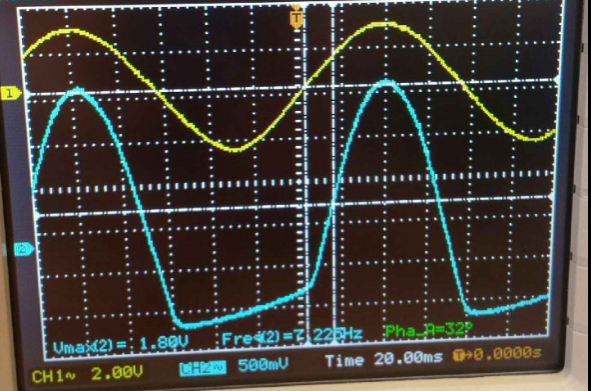
\includegraphics[scale=0.4]{1800mV.png}  
    \caption{$V_{in}= 2.64V$, $f=7.225Hz$, $V_{out} = 1.80V$}
\end{figure}


The group then increased the amplitude of the input voltage to 4.08V. The resulting $V_{out}$ was 2.72V.

\begin{figure}[h]
    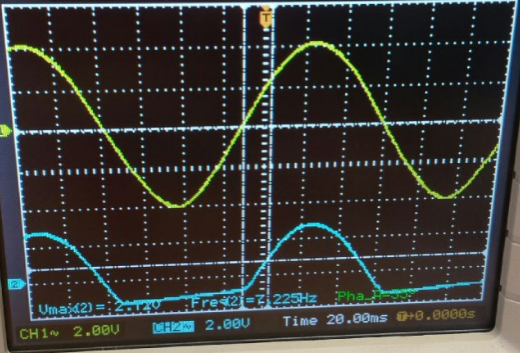
\includegraphics[scale=0.45]{2720mV.png}  
    \caption{$V_{in}= 4.08V$, $f=7.225Hz$, $V_{out}= 2.72V$}
\end{figure}


The group then reset the input voltage to 2.64V and increased the frequency to 75.19Hz. The resulting $V_{out}$ was 1.76V

\begin{figure}[h]
    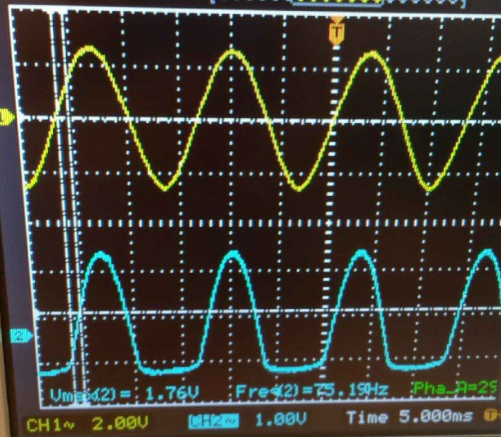
\includegraphics[scale=0.45]{1760mV.png}  
    \caption{$V_{in} = 2.64V$, $f=75.19Hz$, $V_{out}= 1.76V$}
\end{figure}

%fourth frequency: same for higher

The reference voltage added was a 3.065V DC source, constructed in the manner shown in figure (1). 

The input voltage was decreased to 1.48V, and the frequency was set to 7.225Hz. The resulting $V_{out}$ was 460mV.

\begin{figure}[h]
    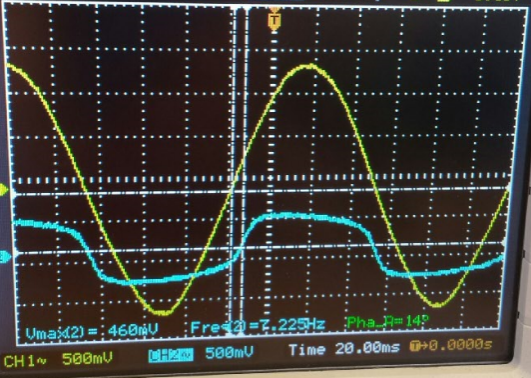
\includegraphics[scale=0.45]{460mV.png}  
    \caption{$V_{in}= 1.48V$, $f=7.225Hz$, $V_{out}= 460mV$}
\end{figure}

%The input voltage and frequency were then set to 2.64V and 731.0mHz respectively. The $V_{out}$ for the diode was 464mV.

%\begin{figure}
%    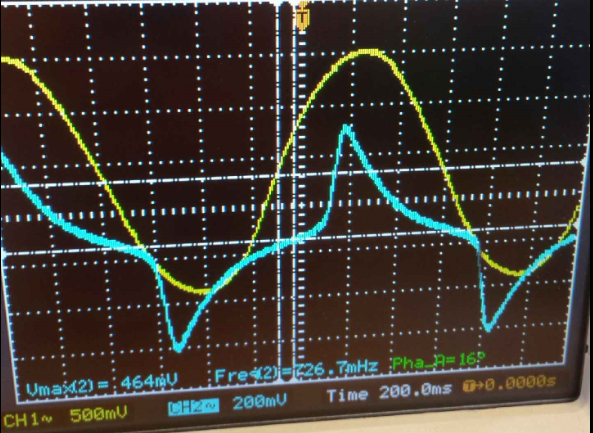
\includegraphics[scale=0.3]{464mV.png}  
%    \caption{$V_{in}$ = 2.64V f=731.0mHz $V_{out}$= 464mV}
%\end{figure}


The group increased the frequency to 74.63Hz and the voltage to 2.64. The resulting $V_{out}$ was 480mV.

\begin{figure}[h]
    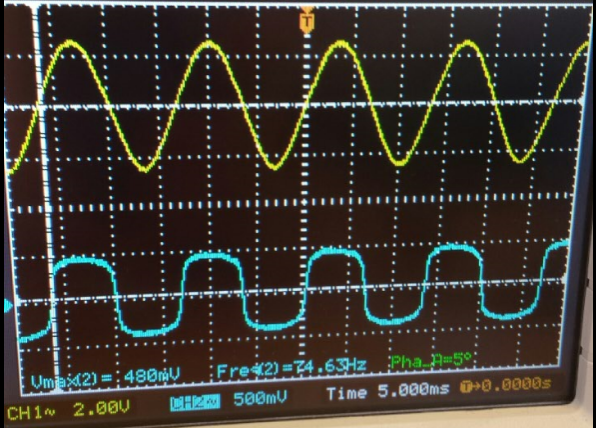
\includegraphics[scale=0.4]{480mV.png}  
    \caption{$V_{in} = 2.64V$, $f=74.63Hz$, $V_{out}= 480mV$}
\end{figure}

The full wave rectifier was built, as in figure (2), using a 98.6k$\Omega$ resistor. %ADD RESISTANCE
\begin{figure}[h]
    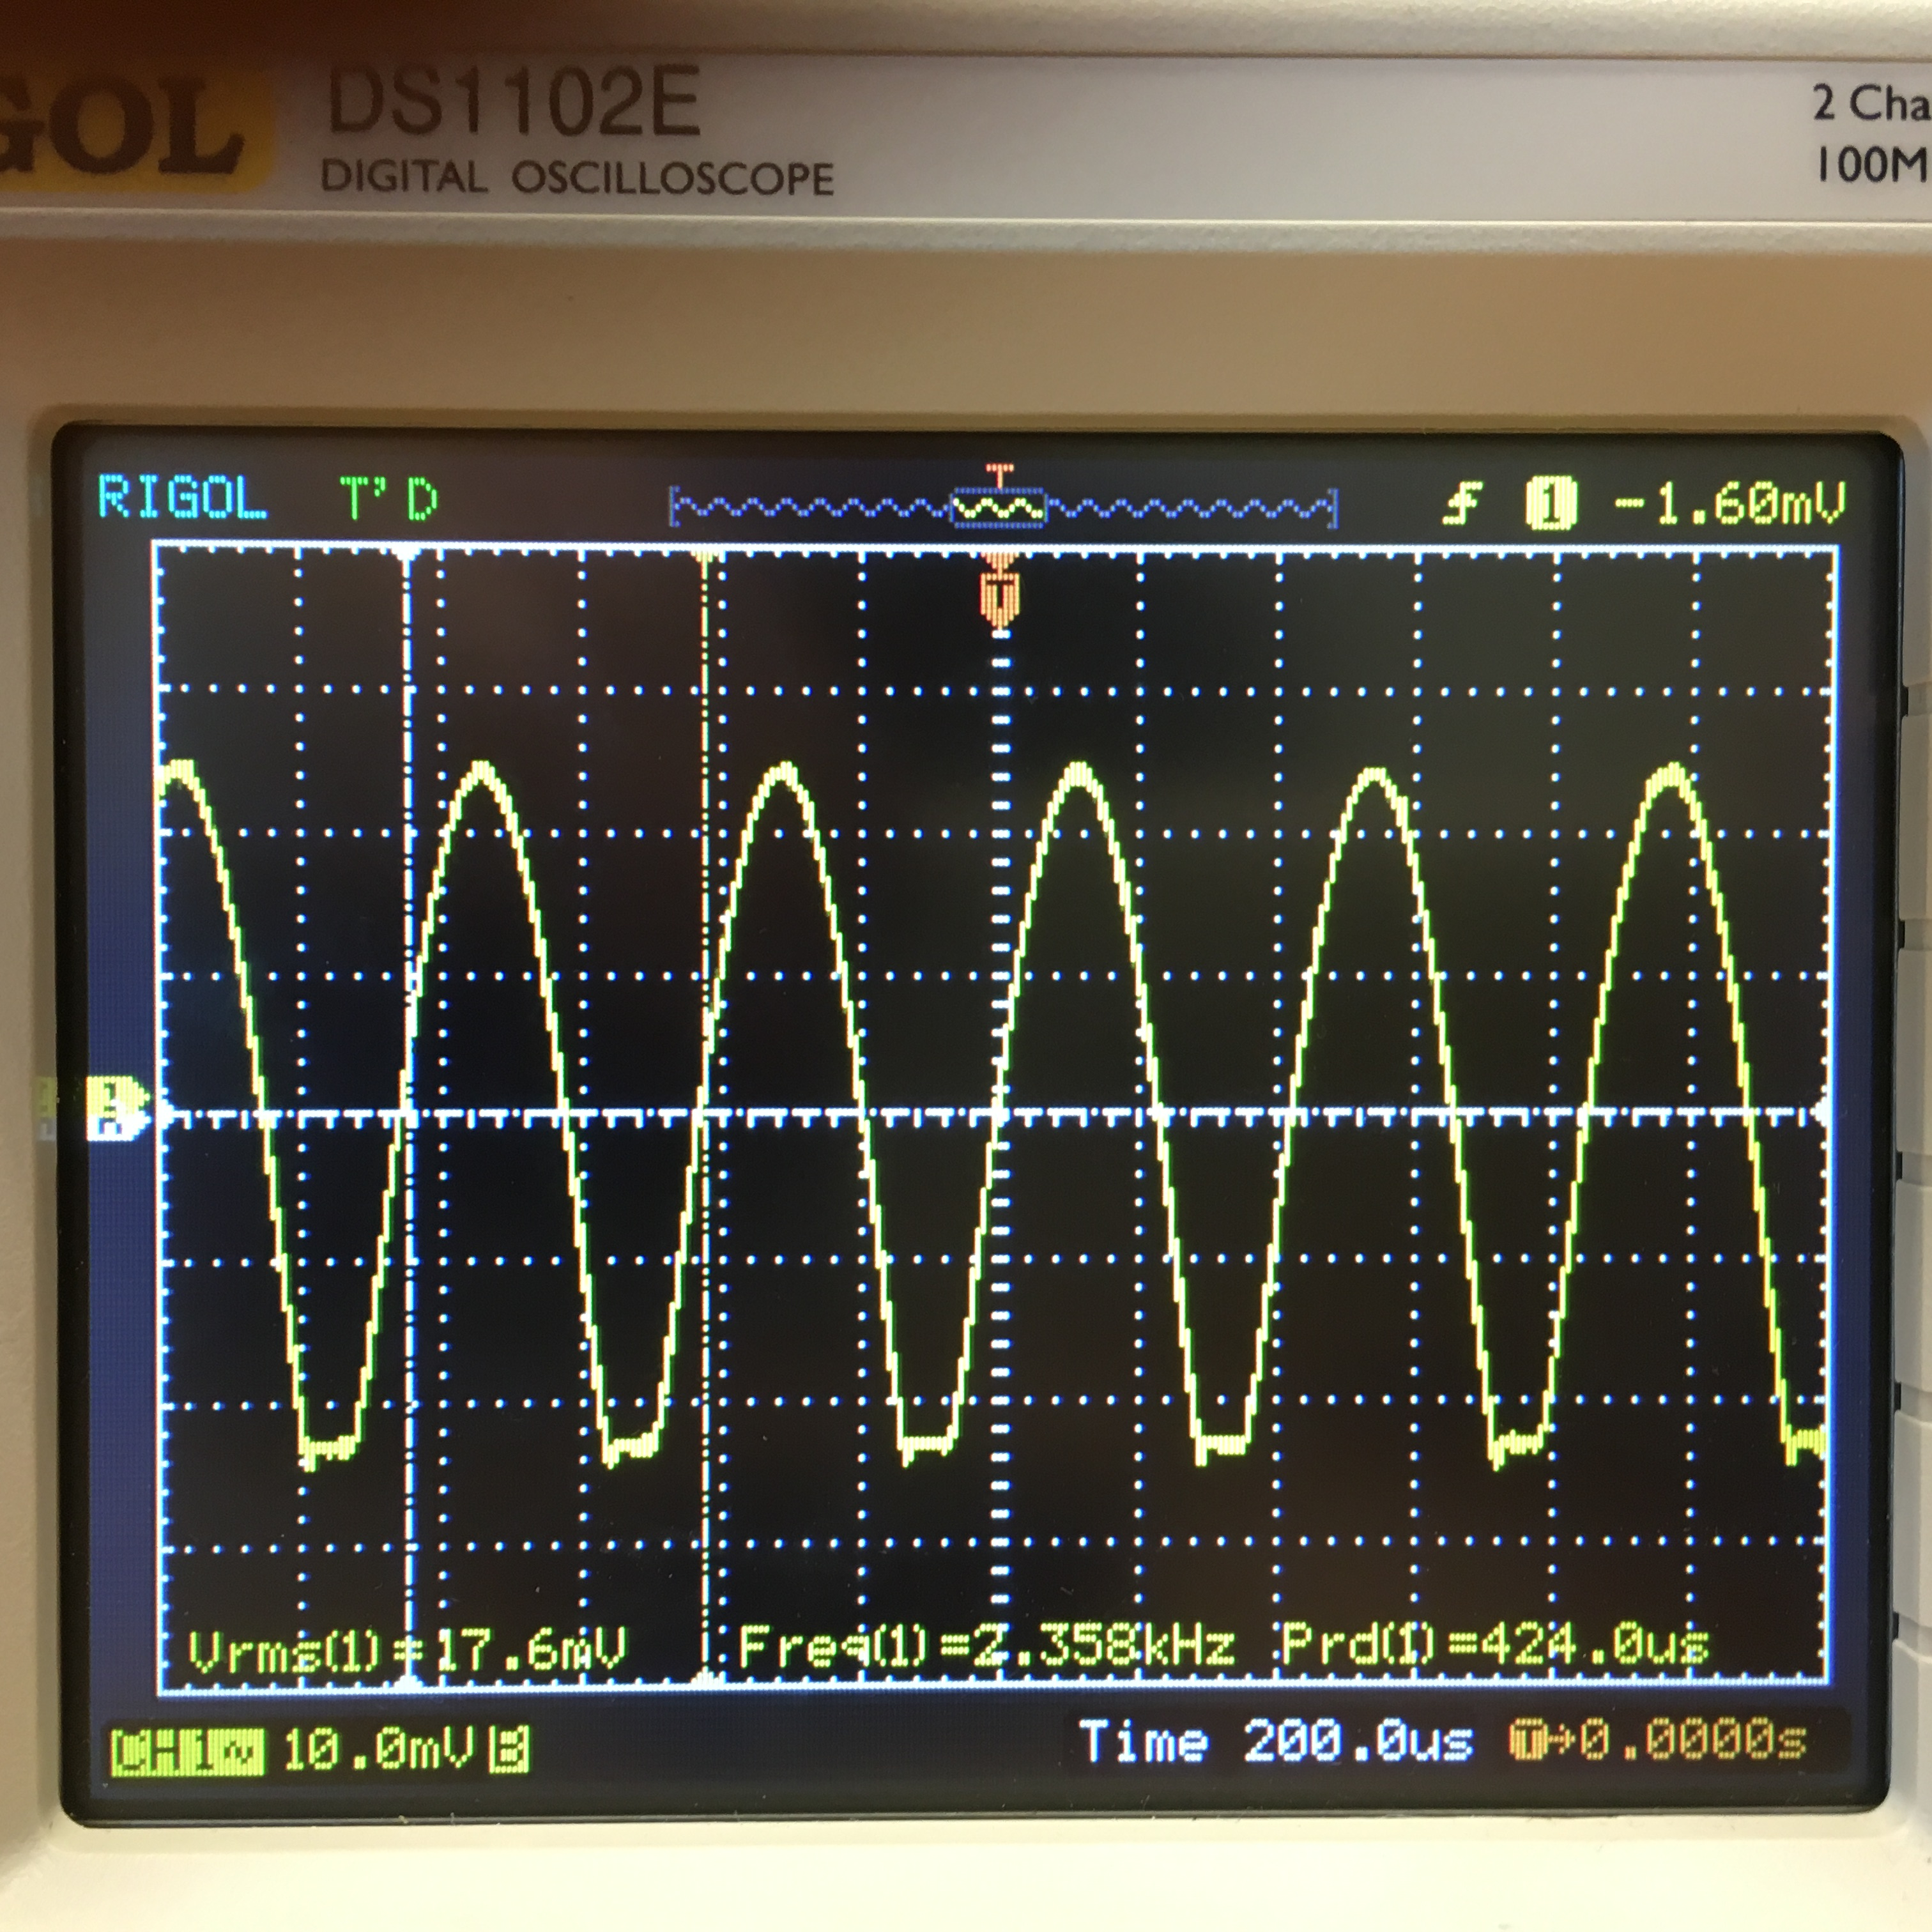
\includegraphics[scale=0.04]{fullbridge1}  
    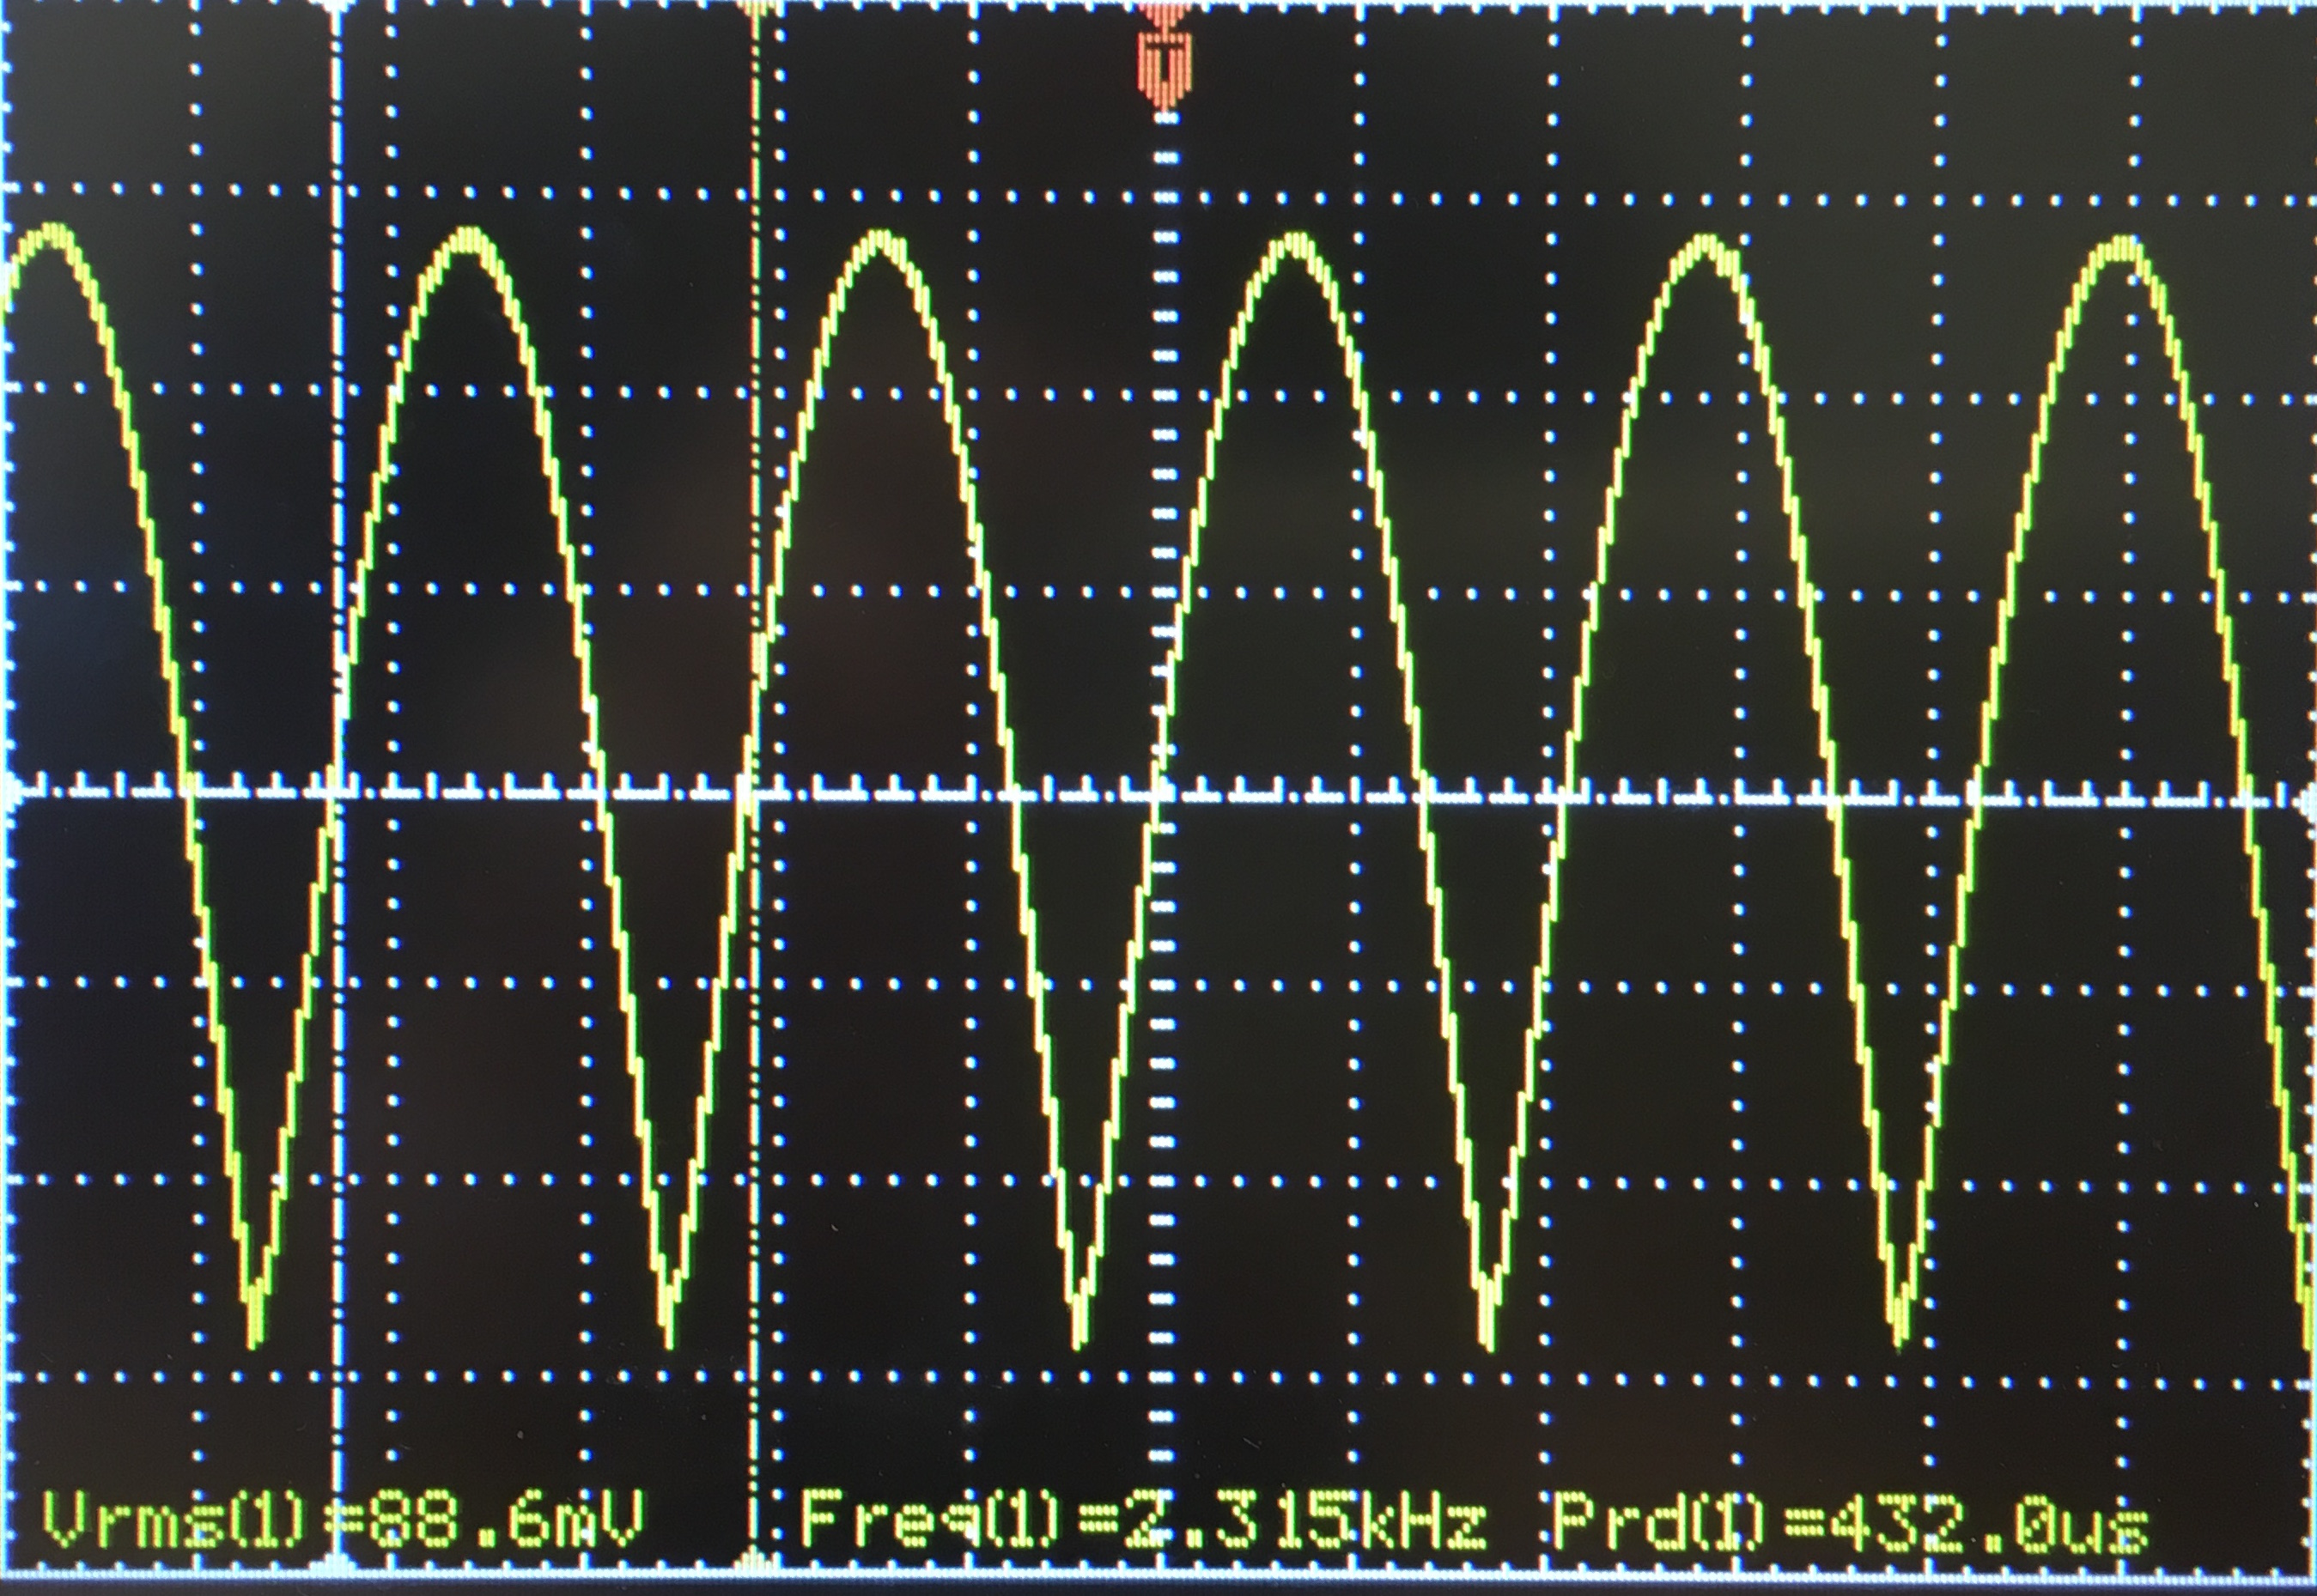
\includegraphics[scale=0.039]{fullbridge2} 
    \caption{Full bridge rectifier at about 2.3kHz, the first with a smaller input voltage, the second with a larger input voltage.}
\end{figure}


The circuit shown in figure (3) was built using a 2.219k$\Omega$ resistor. First, the the Zener diode's behavior was observed as input voltage was varied.
\begin{figure}[h]
    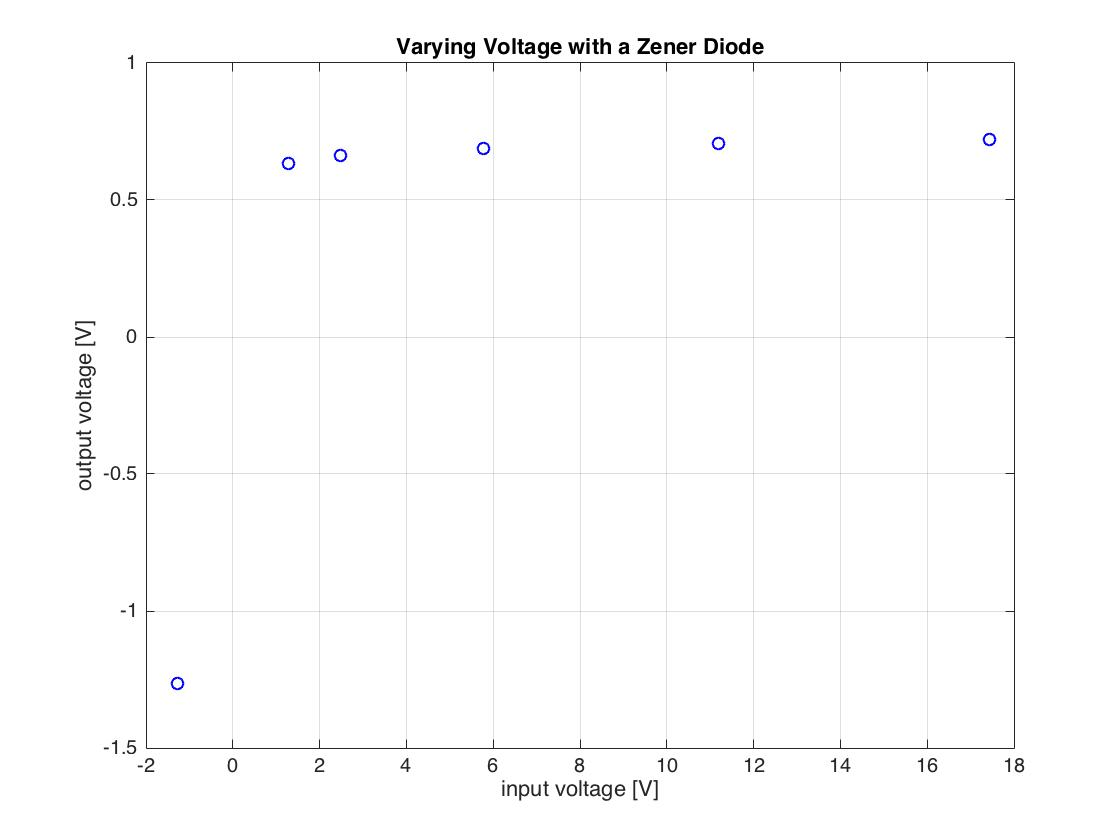
\includegraphics[scale=0.2]{zenerdiode_plot}  
    \caption{Zener diode's response to varying voltage.}
\end{figure}

Two Zener diodes in series in the same direction acted the same as one.

One Zener diode resulted in the clipping of the negative voltage.
\begin{figure}[h]
    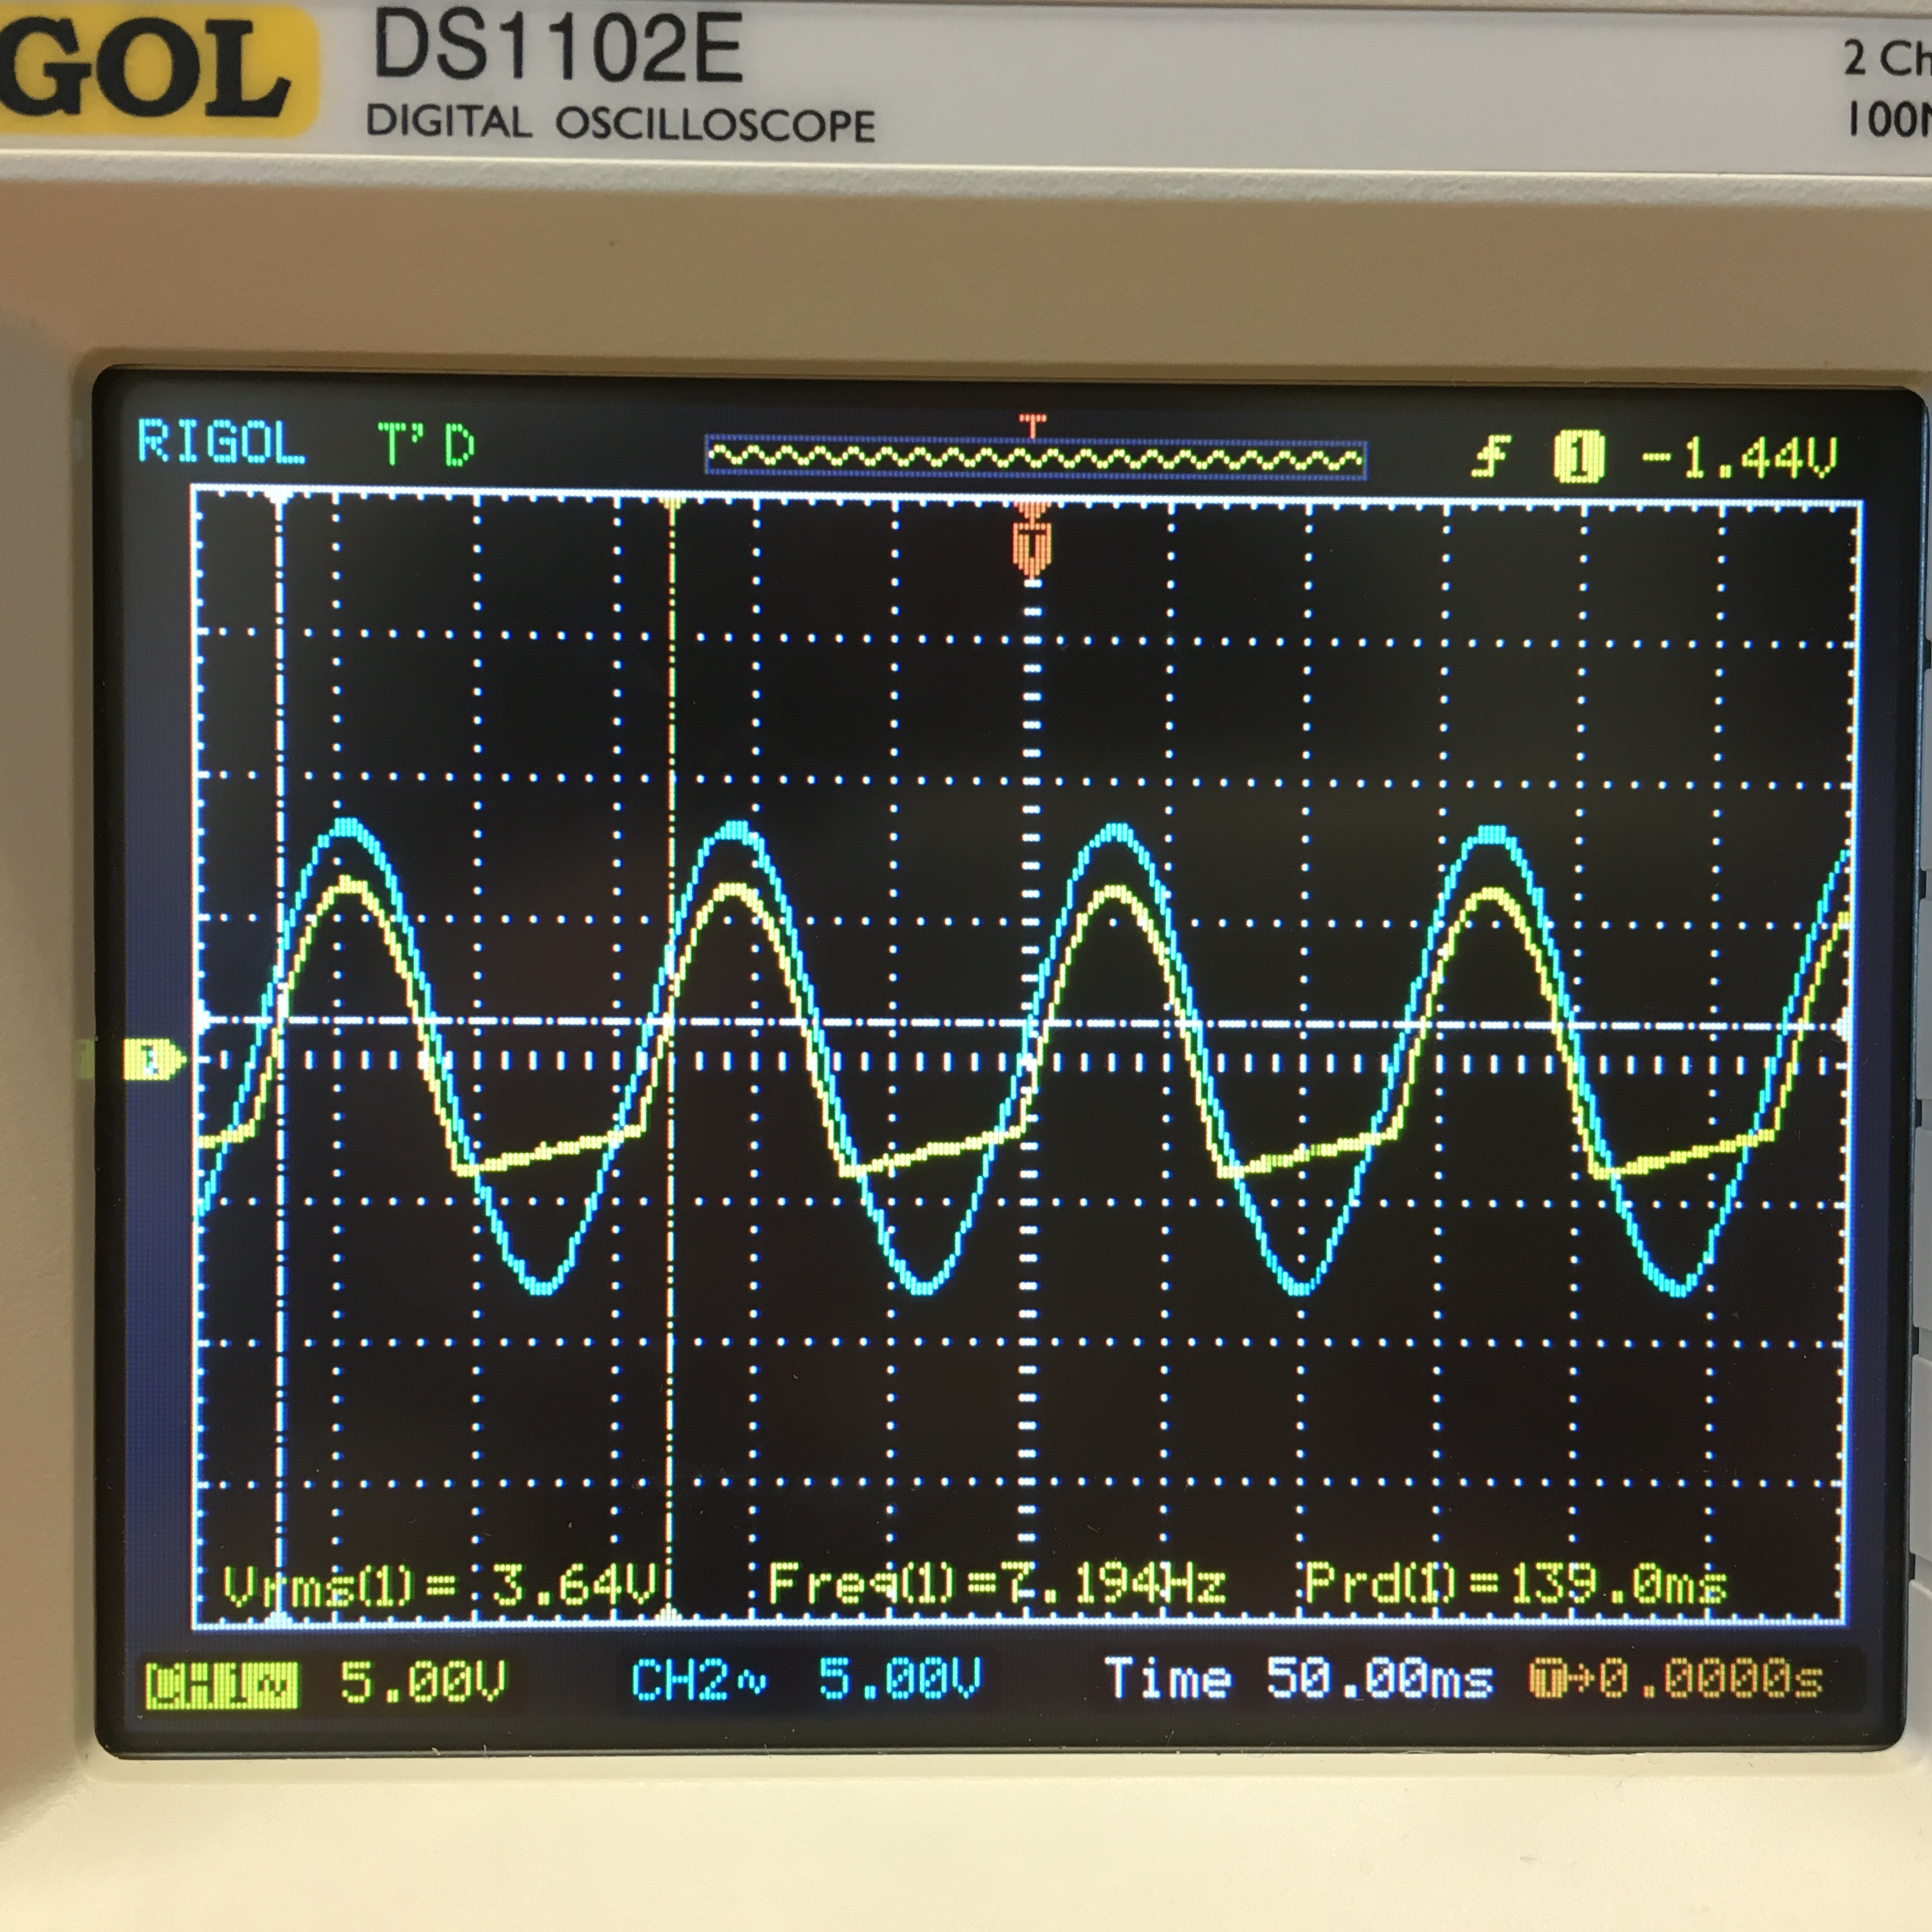
\includegraphics[scale=0.041]{zener2}  
    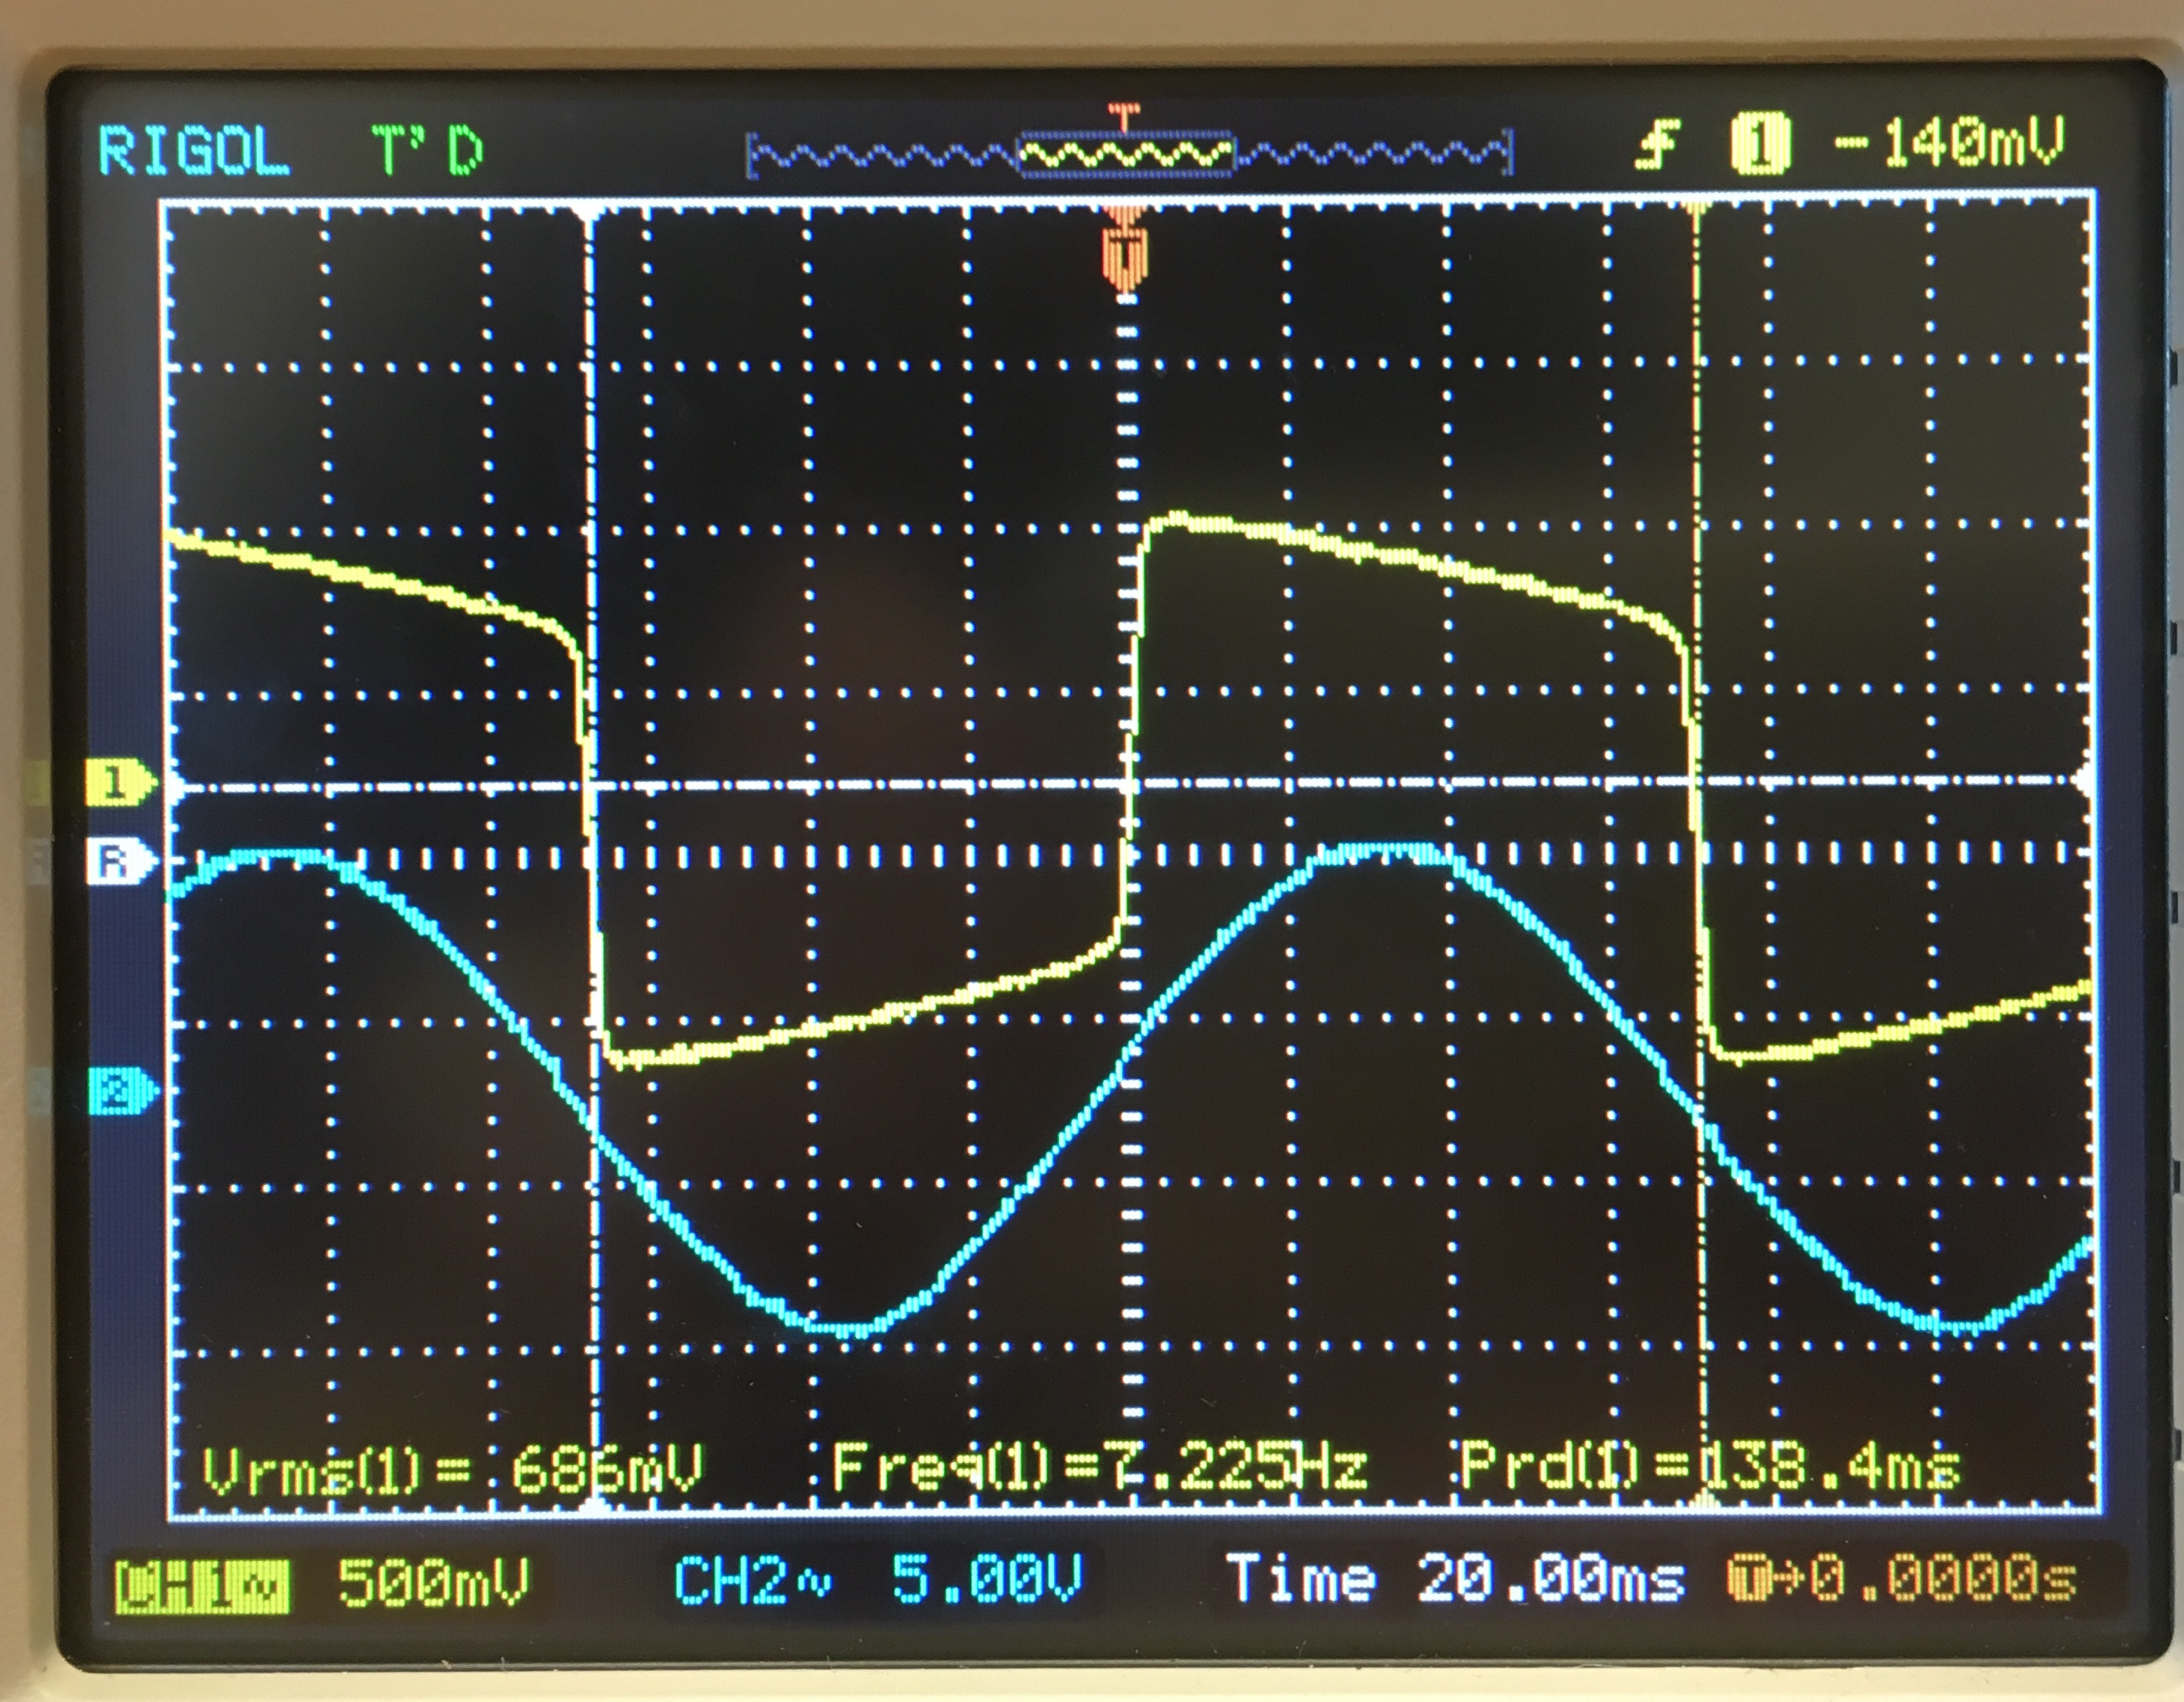
\includegraphics[scale=0.041]{zener1}  
    \caption{Left: single Zener diode clipping negative voltage. Right: two Zener diodes in opposite directions clipping both positive and negative voltage.}
\end{figure}
Two Zener diodes in opposite directions resulted in the clipping of both positive and negative voltages.

%\begin{figure}[h]
%    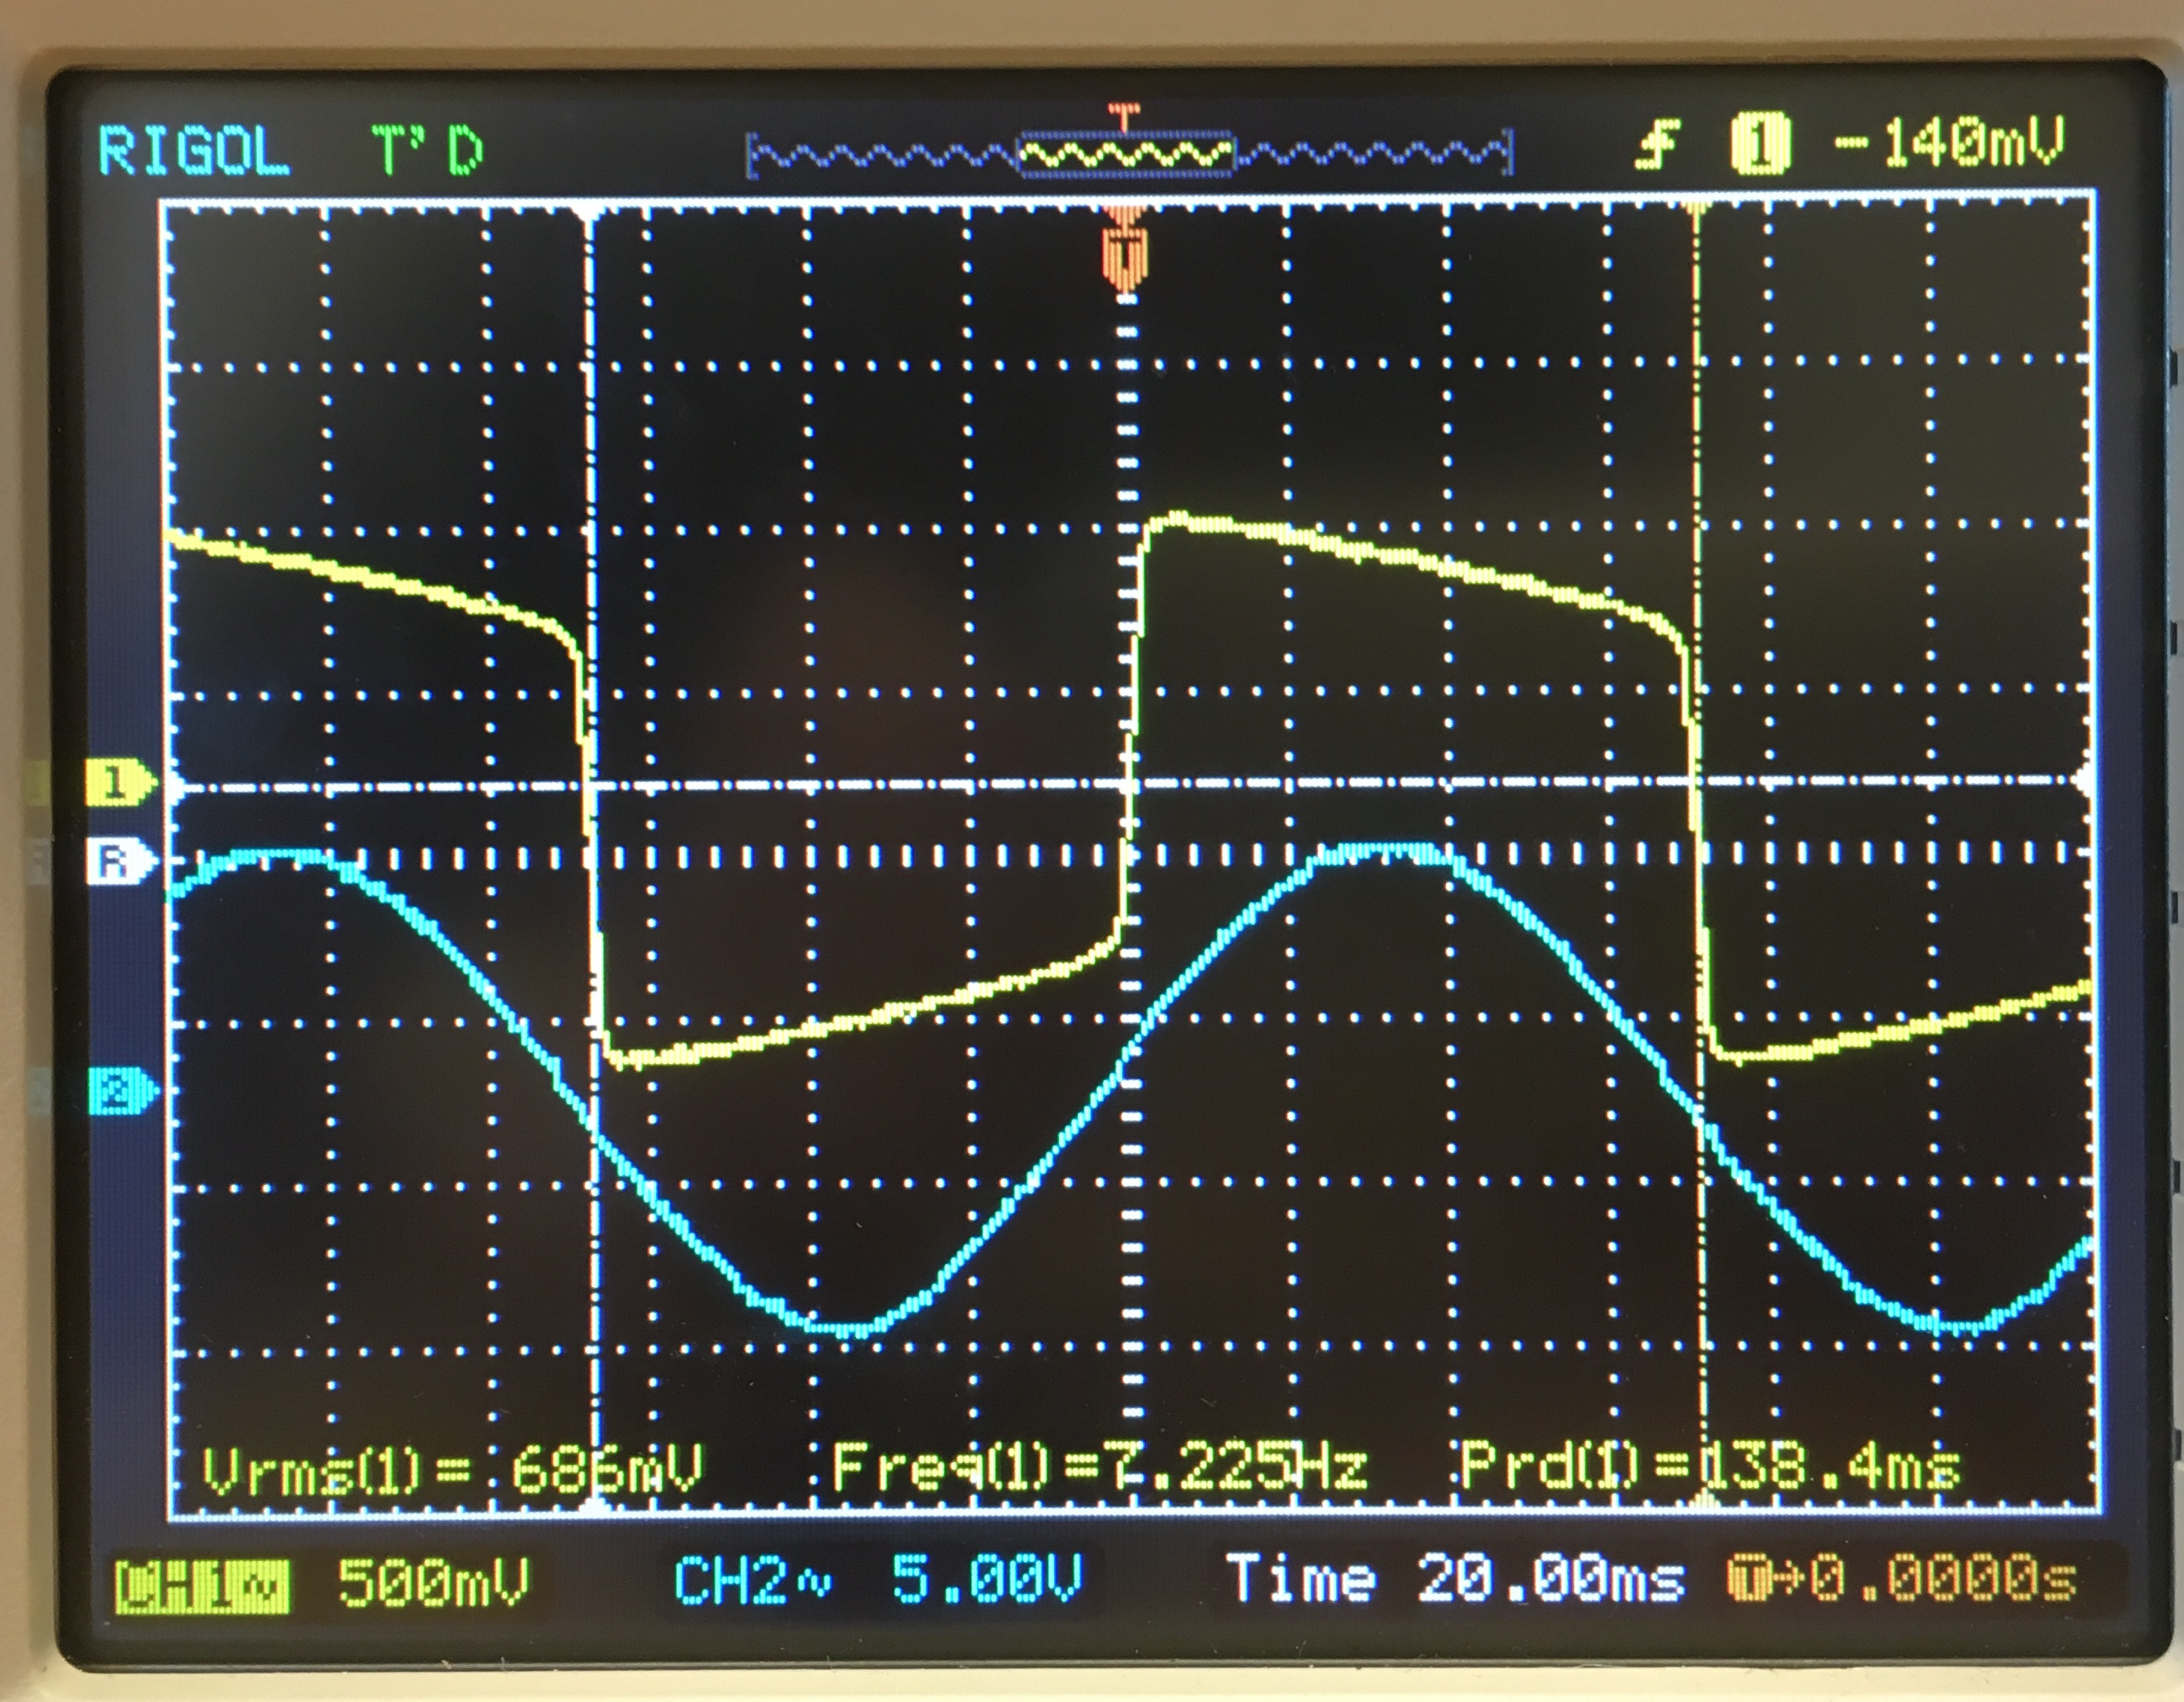
\includegraphics[scale=0.06]{zener1}  
%    \caption{Zener diode clipping positive and negative voltage.}
%\end{figure}


 
\subsection{Analysis}
When only an AC voltage source was connected to the diode and resistor that were in series, the result was half of a sine wave. This was what was expected because the diode only allows current flow in one direction. The current will flow only in the negative direction which will cause the voltage across the oscilloscope to be equal to the diode voltage. When current cannot flow through the diode almost all of the voltage is across the oscilloscope. This means that when the voltage of the input source is positive the voltage across the oscilloscope is equal to the input voltage. 

When the amplitude of the input source was increased, the slight angle of linear portion of the plots appeared to decrease, as the larger amplitude of the positive curve made the slant relatively smaller. As the frequency was increased the plot looked almost like a DC source that was turning on and off because the diode voltage was reached faster, reducing the curve on the bottom of the voltage plot.

When the reference voltage was added, the sinusoidal voltage across the diode became flat on top and bottom, looking much like a square wave. When a negative input voltage was supplied, current flowed through the resistor and the voltage across the diode %this said resistor before, it's supposed to be diode, right?
 was equal to the diode voltage. When the voltage of the input source was positive, the 3.065V from the DC source consumed the input voltage. The input voltage was never greater than 3V, and so the output voltage was 0V. If the voltage of the input had been greater than 3V, then the voltage across the oscilloscope would have been equal to 3V.

When the frequency was increased, the plot flattened out on top and bottom and looked again like a DC input that was flickering up and down by 480mV. This makes sense as the diode was expected to vary between the diode voltage and zero. When frequency was increased the diode voltage was reached more quickly and therefore makes the plot look flatter.

The full wave rectifier, output shown in figure (9), behaved as expected. The output voltage looked like a sine wave where all of the negative values had been turned positive. At lower input voltages, the voltage would stay near zero before continuing with the positive sine wave. This was because it took some time for the voltage to overcome the diode voltage. The effect was less noticeable at larger amplitudes at the same frequency because the voltage gets larger more quickly.

Lastly, the behavior of Zener diodes was also as expected. It let DC voltage through in the positive bias direction the same way a wire would. In the opposite direction, the voltage stayed nearly constant at what must be the Zener voltage, shown in figure (10). With AC voltage applied to a single Zener diode, the negative voltage was clipped. The negative voltage was the reverse bias direction, so when the input voltage was greater than the Zener voltage, only the Zener voltage was output. It was found that two Zener diodes in series in the same direction acted the same as one diode, with a small added voltage drop. When AC voltage was applied to two Zener diodes in series facing opposite directions, both the positive and negative voltages were clipped at the Zener voltage. With two Zener diodes, the voltage is always in the reverse bias direction for one of the diodes. These expected results were consistent with the actual results shown in figure (11).

\section{Conclusion}
The first part of the lab was completed successfully as the group was able to demonstrate that a diode can be used to create close to half of a DC voltage supply. The group discovered that for higher frequency input voltages the plot was more flat on top and bottom. The correct properties of the diode were demonstrated in this part of the lab. When then 3V DC source was added, the results were accurate as the voltage varied between zero and the diode voltage. This is what would have been expected for input voltages below 3V. Results for voltages above 3V were not obtained. This could be done in future labs.

A full wave rectifier was successfully constructed. Its behavior was as expected, creating an all positive voltage output by inverting the negative input voltage. 

The Zener diode portion of the lab was also successful. The Zener voltage behavior was observed by measuring the output voltage while varying the DC input voltage. Then the clipping effect of the Zener diode on half of the waveform was observed by providing a single Zener diode with an AC voltage input. Then, using two diodes in opposite bias directions, the both the positive and negative output voltages were clipped.

Overall, the lab was completed with a large degree of success.



\end{document}

